\begin{enumerate}[label=\thechapter.\arabic*,ref=\thechapter.\theenumi]
\item A sinusoidal message signal having root mean square value of 4V and frequency of 1 kHz fed to a phase modulator with phase deviation constant 2 rad/volt. If the carrier signal is $c\brak{t} = 2\cos \brak{2\pi 10^6 t}$, the maximum instantaneous frequency of the phase modulated signal (rounded off to one decimal place) is \rule{1cm}{0.05mm} Hz. \hfill(GATE 2021 EC)\\
\solution\\
 \iffalse
\let\negmedspace\undefined
\let\negthickspace\undefined
\documentclass[journal,12pt,onecolumn]{IEEEtran}
\usepackage{cite}
\usepackage{amsmath,amssymb,amsfonts,amsthm}
\usepackage{algorithmic}
\usepackage{graphicx}
\usepackage{textcomp}
\usepackage{xcolor}
\usepackage{txfonts}
\usepackage{listings}
\usepackage{enumitem}
\usepackage{mathtools}
\usepackage{gensymb}
\usepackage{comment}
\usepackage[breaklinks=true]{hyperref}
\usepackage{tkz-euclide} 
\usepackage{tikz}
\usepackage{circuitikz}
%\usetikzlibrary{circuits.ee.IEC}
\usepackage{listings}
\usepackage{gvv} 
\usepackage{caption}
\def\inputGnumericTable{}                   

%\usepackage[latin1]{inputenc}                                
\usepackage{color}                                            
\usepackage{array}                                            
\usepackage{longtable}                                       
\usepackage{calc}                                             
\usepackage{multirow}                                         
\usepackage{hhline}                                           
\usepackage{ifthen}                                           
\usepackage{lscape}
\usepackage{tikz}
\usepackage{circuitikz}

\newtheorem{theorem}{Theorem}[section]
\newtheorem{problem}{Problem}
\newtheorem{proposition}{Proposition}[section]
\newtheorem{lemma}{Lemma}[section]
\newtheorem{corollary}[theorem]{Corollary}
\newtheorem{example}{Example}[section]
\newtheorem{definition}[problem]{Definition}
\newcommand{\BEQA}{\begin{eqnarray}}
\newcommand{\EEQA}{\end{eqnarray}}
\newcommand{\define}{\stackrel{\triangle}{=}}
\theoremstyle{remark}
\newtheorem{rem}{Remark}

\begin{document}

\bibliographystyle{IEEEtran}
\vspace{3cm}

\title{GATE: EE - 59.2022}
\author{EE23BTECH11013 - Avyaaz$^{*}$% <-this % stops a space 
}
\maketitle
% \newpage
% \bigskip

\renewcommand{\thefigure}{\arabic{figure}}
\renewcommand{\thetable}{\arabic{table}}

\large\textbf{\textsl{Question:}}
For the ideal AC-DC rectifier circuit shown in the figure below, the load current
magnitude is $I_{dc}$ = $15$ A and is ripple free. The thyristors are fired with a delay angle
of 45\degree
. The amplitude of the fundamental component of the source current, in
amperes, is \_\_\_\_\_\_\_\_{\em (Round off to 2
decimal places)}. \hfill(GATE 59 EE 2022)
\begin{figure}[!h]
\centering
\begin{circuitikz}[american voltages]
    \draw (0,0) node[op amp] (opamp) {};
    \draw (opamp.+) node[above]{$v_{+}$} to (-2,-0.5);
    \draw (opamp.-) node[above]{$v_{-}$} to (-2, 0.5);
    \draw (opamp.out) to (2, 0)node[right]{$v_{out}$};
    \draw (opamp.down) to (-0.1, -1) node[below]{$-v_{EE}$};
    \draw (opamp.up) to (-0.1, 1)node[above]{$+v_{DD}$};
    \draw (-2,0.5) to [R, l_=$R_1$](-3,0.5) to (-3.5, 0.5) to [V, l_=$0.1v$] (-3.5, -2) node[ground]{};
    \draw (-2, -0.5) to [R, l=$R_2$] (-2, -2) node[ground]{};
    \draw (-1.5,0.5) to (-1.5, 2) to [C, l=$C_1$] (1.5, 2) to (1.5, 0);
\end{circuitikz}

\end{figure}

\solution
\fi
\begin{table}[htbp]
\setlength{\extrarowheight}{4pt}
\setlength{\tabcolsep}{3pt}
\centering
\begin{tabular}{|c|c|c|}
\hline
\textbf{Parameter} & \textbf{Description}&\textbf{Value}\\
\hline 
$I_{dc}$& Load current & $15$A  \\
\hline
$\alpha$ &Firing angle&$45\degree$ \\
\hline
\end{tabular}

\caption{}
\label{tab:inputs.EE.59.2022}
\end{table}
% It is a Single phase symmetrical semi-converter.
% \begin{enumerate}[label={\roman*)}]
%     \item Load current magnitude $\brak{I_{dc}}$ = $15$A
%     \item Firing angle $\brak{\alpha} = 45\degree$
% \end{enumerate}
A symmetrical single phase semi converter is shown below,

\begin{figure}[!h]
\centering
    \begin{circuitikz}[scale = 0.8]
      \draw (-0.8,0.8) -- (-0.8,0.8) node[above]{$+$};
    \draw (0,2) to[sV,l=$V_s$] (0,-1);
     \draw (-0.8,0) -- (-0.8,0) node[below]{$-$};
    \draw (0,2) -- (2,2);
    \draw (2,2) -- (2,1);
    \draw (2,1) -- (3,1);
     \draw (3,1) to [thyristor] (3,3);
     \node at (2.4,2.3) {$T_1$};
    \draw (3,3) -- (5,3);
    \draw (5,1) to [thyristor] (5,3);
     \node at (4.4,2.3) {$T_2$};
    \draw (5,3) -- (7,3);
    \draw (7,3) to[resistor](7,1);
    \draw (7,1) -- (7,0);
    \draw(7,0) to [L](7,-2);
    \draw (7,-2) -- (3,-2);

    \draw (0, -1) -- (2,-1);
    \draw (2,-1) -- (2,0.4);
    \draw (2,0.4) -- (5,0.4);
    \draw (3,-2) to [Do] (3,0.4);
    \node at (3.8,-1) {$D_1$};
    \draw (3,0.4) -- (3,1);
    \draw (5,-2) to [Do] (5,0.4);
    \node at (5.8,-1) {$D_2$};
    \draw (5,0.4) -- (5,1);

     \draw[->] (6.5, 2) -- (6.5, 1) node[midway, left]{$I_{dc}$};
          \draw[->] (0.5, 2) -- (1, 2) ;
          \node at (1,1.6) {$I_s$};
          \node at (7.4,2) {$R$};
          \node at (7.4,-1.1) {$L$};

     \draw (8,2.8) -- (8,2.8) node[above]{$+$};
     \draw[->] (8,0.8) -- (8,2.8);
     \node at (8,0.5) {$V_o$};
     \draw[->] (8,0.2) -- (8,-1.8);
     \draw (8,-1.8) -- (8,-1.8) node[below]{$-$};
        \end{circuitikz}

\end{figure}

The Fourier series representation of supply current is given by:
\begin{align}
    i_s(t) = a_o +\sum_{n=1}^{\infty}C_n\sin({n\omega t} + \theta_n)\label{eq:gen_i_s}
\end{align}
 where,
 \begin{align}
 a_o &= \frac{1}{2\pi} \int_{0}^{2\pi} i_s(t)d\omega t \\
     C_n &= \sqrt{a_n^2 + b_n ^2}\label{eq:bino_coeff}\\
     \theta_n &= \tan^{-1}\left({\frac{a_n}{b_n}}\right)\label{eq: theta}
 \end{align}
\begin{align}
  \implies  a_o &= \frac{1}{2\pi}\int_{\alpha}^{\pi} I_o d\omega t - \int_{\pi + \alpha}^{2\pi} I_o d\omega t = 0\\
 \implies   a_n &= \frac{1}{\pi} \int_{\alpha}^{\pi}I_o\cos n\omega t d\omega t - \int_{\pi + \alpha}^{2\pi} I_o\cos{n\omega td\omega t}\\
 a_n &= 
 \begin{cases}
    \frac{-2I_o}{n\pi}\sin{n\alpha} & \text{for } n = 1,3,5...\\
     0 &\text{for } n = 2,4.....
    \end{cases}\\
 \implies   b_n &= \frac{1}{\pi}\int_{\alpha}^{\pi}I_o\sin n\omega t d\omega t - \int_{\pi + \alpha}^{2\pi} I_o\sin{n\omega td\omega t} \\
 b_n &= 
 \begin{cases}
     \frac{2I_o}{n\pi}\left(1 + \cos{n\alpha}\right) &\text{for } n = 1,3,5...\\
     0 &\text{for } n = 2, 4....
    \end{cases}
    \end{align}
From \eqref{eq:bino_coeff}:
\begin{align}
  \therefore  C_n &= \frac{2\sqrt{2}I_o}{n\pi}\left(\sqrt{1 + \cos{n\alpha}}\right)\\
  \implies  C_n &= \frac{4I_o}{n\pi}\cos{\frac{n\alpha}{2}}\label{eq:final_bino}
\end{align}
From \eqref{eq: theta}:
\begin{align}
    \theta_n &= \tan^{-1}\left(\frac{-\sin{n\alpha}}{1 + \cos{n\alpha}}\right)\\
    \implies \theta_n &= \frac{-n\alpha}{2}\label{eq:final_theta}
\end{align}

From \eqref{eq:gen_i_s},\eqref{eq:final_bino} and \eqref{eq:final_theta}:
\begin{align}
I_{s}(t) = \sum_{n=1,3,5...}^{\infty} \frac{4I_{o}}{n\pi}\cos{\frac{n\alpha}{2}}\sin{\left(n\omega t - \frac{n\alpha}{2}\right)}
\end{align}
% \begin{align}
% I_{s}(t) = \sum_{n=1,3,5...}^{\infty} \frac{4I_{dc}}{n\pi}\cos{\frac{n\alpha}{2}}\sin{\left(n\omega t - \frac{n\alpha}{2}\right)}
% \end{align}


% \begin{tikzpicture}[scale=1]
%     \draw[->] (0,0) -- (10,0) node[right] {$\omega t$};
%     \draw[->] (0,-2) -- (0,2) node[above] {$y$};
%     \draw[domain=0:10, smooth, variable=\x, black] plot ({\x},{sin(deg(\x))});
%     \foreach \x/\xtext in {1.57/\frac{\pi}{2},3.14/\pi,4.71/\frac{3\pi}{2},6.28/2\pi,7.85/\frac{7\pi}{2}} {
%         \draw (\x cm,0) -- (\x cm,0.1) node[below] {$\xtext$};
%     }
%     \foreach \y in {-1,1} {
%         \draw (1pt,\y cm-1.5) -- (-1pt,\y cm-1.5) node[left] {$\y$};
%     }
% \end{tikzpicture}

\begin{figure}[!h]
    \centering
    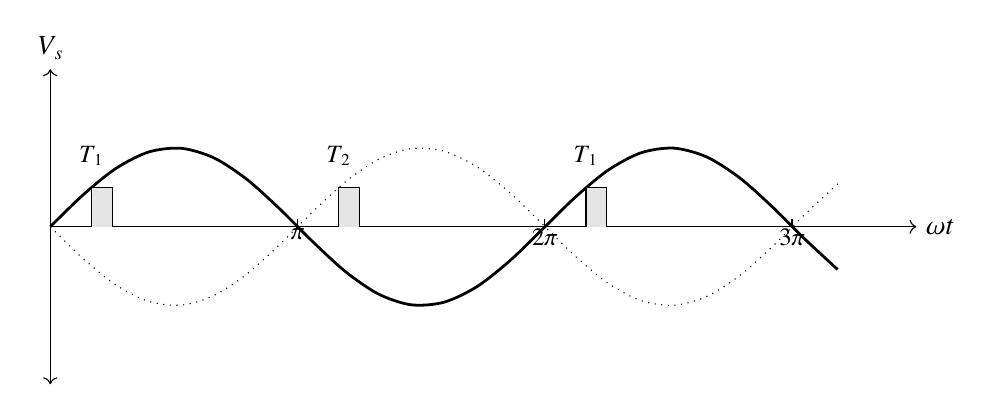
\begin{tikzpicture}[scale=1]
    \draw[->] (0,0) -- (11,0) node[right] {$\omega t$};
    \draw[<->] (0,-2) -- (0,2) node[above] {$V_s$};
    \draw[domain=0:10, smooth, variable=\x, black,line width=1pt] plot ({\x},{sin(deg(\x))});
    \draw[dotted,domain=0:10, smooth, variable=\x, black] plot ({\x},{-sin(deg(\x))});
    \foreach \x/\xtext in {3.14/\pi,6.28/2\pi,9.42/3\pi} {
        \draw (\x cm,0) -- (\x cm,0.1) node[below] {\small$\xtext$};
    }

\fill[gray!20] (0.5233,0) -- (0.5233,0.5) -- (0.785,0.5) -- (0.785,0) -- cycle;
    \fill[gray!20] (3.6633,0) -- (3.6633,0.5) -- (3.925,0.5) -- (3.925,0) -- cycle;
    \fill[gray!20] (6.8033,0) -- (6.8033,0.5) -- (7.065,0.5) -- (7.065,0) -- cycle;

    \draw (0.5233,0) -- (0.5233,0.5);
    \draw (0.5233,0.5) -- (0.785,0.5);
    \draw (0.785,0.5) -- (0.785,0);

    \draw (3.6633,0) -- (3.6633,0.5);
    \draw (3.6633,0.5) -- (3.925,0.5);
    \draw (3.925,0.5) -- (3.925,0);

    \draw (6.8033,0) -- (6.8033,0.5);
    \draw (6.8033,0.5) -- (7.065,0.5);
    \draw (7.065,0.5) -- (7.065,0);


     \node at (0.5233,0.9) {\small$T_1$};
     \node at (3.6633,0.9) {\small$T_2$};
     \node at (6.8033,0.9) {\small$T_1$};
\end{tikzpicture}
\end{figure}
\begin{figure}[!h]
    \centering
    \begin{tikzpicture}[scale=1]
    \draw[->] (0,0) -- (11,0) node[right] {$\omega t$};
    \draw[<->] (0,-2) -- (0,2) node[above] {$V_o$};
    \draw[domain=0.5233:3.14, smooth, variable=\x, black,line width=1pt] plot ({\x},{sin(deg(\x))});
    \draw[domain=3.6633:6.28, smooth, variable=\x, black,line width=1pt] plot ({\x},{-sin(deg(\x))});
    \draw[domain=6.8033:9.42, smooth, variable=\x, black,line width=1pt] plot ({\x},{sin(deg(\x))});

    \foreach \x/\xtext in {0.5233/\alpha, 3.14/\pi,4/\pi + \alpha ,6.28/2\pi,7.2/2\pi + \alpha,9.42/3\pi}{
        \draw (\x cm,0) -- (\x cm,0) node[below] {\small $\xtext$};
    }

     \draw [line width=1pt](0,0)--(0.5233,0);
    \draw [line width=1pt](0.5233,0) -- (0.5233,0.5);
    \draw[line width=1pt](3.14,0)-- (3.6633,0);
    \draw[line width=1pt] (3.6633,0) -- (3.6633,0.5);
    \draw [line width=1pt](6.28,0)--(6.8033,0);
    \draw [line width=1pt](6.8033,0) -- (6.8033,0.5);

    \node at (0.25,0.6){\small$T_2$};
    \node at (0.25,0.2){\small$D_2$};
     \node at (3.4,0.6){\small$T_1$};
    \node at (3.4,0.2){\small$D_1$};
    \node at (6.4,0.6){\small$T_2$};
    \node at (6.4,0.2){\small$D_2$};

    \node at (1.57,0.4){\small $T_1D_2$};
    \node at (4.71,0.4){\small $T_2D_1$};
    
\end{tikzpicture}
\end{figure}
\begin{figure}[!h]
    \centering
    \begin{tikzpicture}[scale=1]
    \draw[->] (0,0) -- (11,0) node[right] {$\omega t$};
    \draw[<->] (0,-2) -- (0,2) node[above] {$i_{T_1}$};
   
    \foreach \x/\xtext in {0.5233/\alpha,4/\pi + \alpha,7.2/2\pi + \alpha,10/3\pi + \alpha}{
        \draw (\x cm,0) -- (\x cm,0) node[below] {\small $\xtext$};
    }
     \draw [line width=1pt](0,0)--(0.5233,0);
    \draw [line width=1pt](0.5233,0) -- (0.5233,1);
    \draw[line width=1pt](0.5233,1)-- (3.6633,1);
    \draw[line width=1pt] (3.6633,1) -- (3.6633,0);
    \draw[line width=1pt] (3.6633,0) -- (6.8033,0);
    \draw [line width=1pt](6.8033,0)--(6.8033,1);
    \draw [line width=1pt](6.8033,1) -- (9.948,1);
     \draw [line width=1pt] (9.948,1) -- (9.948,0);

     \draw[dotted,domain=0:10, smooth, variable=\x, black] plot ({\x},{1});
     \node at (0.4,1.2) {\small $I_{DC}$};
\end{tikzpicture}
\end{figure}
\begin{figure}[!h]
    \centering
    \begin{tikzpicture}[scale=1]
    \draw[->] (0,0) -- (11,0) node[right] {$\omega t$};
    \draw[<->] (0,-2) -- (0,2) node[above] {$i_{s}$};
   

    \draw [line width=1pt](0.5233,0) -- (0.5233,1);
    \draw[line width=1pt](0.5233,1)-- (3.14,1);
    \draw[line width=1pt](3.14,1)-- (3.14,0);
    \draw[line width=1pt] (3.14,0) -- (3.6633,0);
    \draw[line width=1pt] (3.6633,0) -- (3.6633,-1);
    \draw[line width=1pt] (3.6633,-1) -- (6.28,-1);
    \draw[line width=1pt]  (6.28,-1) -- (6.28,0);
    \draw[line width=1pt] (6.28,0) -- (6.8033,0);
    \draw [line width=1pt](6.8033,0)--(6.8033,1);
    \draw [line width=1pt](6.8033,1) -- (9.42,1);
     \draw [line width=1pt] (9.42,1) -- (9.42,0);
     \draw [line width=1pt] (9.42,0) -- (9.948,0);

     \draw[dotted,domain=0:10, smooth, variable=\x, black] plot ({\x},{1});
     \node at (0.4,1.2) {\small $I_{DC}$};
    
\end{tikzpicture}
\end{figure}

From \tabref{tab:inputs.EE.59.2022}:
\begin{align}
   (I_{s_1})_{peak} &= \frac{4I_{dc}}{\pi}\cos{\left(\frac{\alpha}{2}\right)}\\
    &= \frac{4 \times 15 }{\pi}\times \cos{\frac{45 \degree}{2}}\\
    &=17.64 A 
\end{align}

%\end{document}

\pagebreak
\item Two discrete-time linear time-invarient systems with impulse responses $h_1[n]=\delta[n-1]+\delta[n+1]$ and $h_2[n]=\delta[n]+\delta[n-1]$ are connected in cascade, where $\delta[n]$ is the Kronecker delta. The impulse response of the cascaded system is   \\
\begin{enumerate}[label=(\alph*)]
    \item $\delta[n-2]+\delta[n+1]$
    \item $\delta[n-1]\delta[n]+\delta[n+1]\delta[n-1]$
    \item $\delta[n-2]+\delta[n-1]+\delta[n]+\delta[n+1]$
    \item $\delta[n]\delta[n-1]+\delta[n-2]\delta[n+1]$
\end{enumerate} \hfill(GATE 2021 EE)\\
\solution
% \iffalse
\let\negmedspace\undefined
\let\negthickspace\undefined
\documentclass[journal,12pt,twocolumn]{IEEEtran}
\usepackage{cite}
\usepackage{amsmath,amssymb,amsfonts,amsthm}
\usepackage{algorithmic}
\usepackage{graphicx}
\usepackage{textcomp}
\usepackage{xcolor}
\usepackage{pgfplots}
\usepackage{txfonts}
\usepackage{listings}
\usepackage{enumitem}
\usepackage{mathtools}
\usepackage{gensymb}
\usepackage{comment}
\usepackage[breaklinks=true]{hyperref}
\usepackage{tkz-euclide} 
\usepackage{listings}
\usepackage{gvv}                                        
\def\inputGnumericTable{}                                 
\usepackage[latin1]{inputenc}                                
\usepackage{color}                                            
\usepackage{array}                                            
\usepackage{longtable}                                       
\usepackage{calc}                                             
\usepackage{multirow}                                         
\usepackage{hhline}                                           
\usepackage{ifthen}                                           
\usepackage{lscape}

\newtheorem{theorem}{Theorem}[section]
\newtheorem{problem}{Problem}
\newtheorem{proposition}{Proposition}[section]
\newtheorem{lemma}{Lemma}[section]
\newtheorem{corollary}[theorem]{Corollary}
\newtheorem{example}{Example}[section]
\newtheorem{definition}[problem]{Definition}
\newcommand{\BEQA}{\begin{eqnarray}}
\newcommand{\EEQA}{\end{eqnarray}}
\newcommand{\define}{\stackrel{\triangle}{=}}
\theoremstyle{remark}
\newtheorem{rem}{Remark}
\begin{document}
\parindent 0px
\bibliographystyle{IEEEtran}
\title{GATE: EE - 7.2021}
\author{EE22BTECH11219 - Rada Sai Sujan$^{}$% <-this % stops a space
}
\maketitle
\newpage
\bigskip
\section*{Question}
Two discrete-time linear time-invarient systems with impulse responses $h_1[n]=\delta[n-1]+\delta[n+1]$ and $h_2[n]=\delta[n]+\delta[n-1]$ are connected in cascade, where $\delta[n]$ is the Kronecker delta. The impulse response of the cascaded system is   \\
\begin{enumerate}[label=(\alph*)]
    \item $\delta[n-2]+\delta[n+1]$
    \item $\delta[n-1]\delta[n]+\delta[n+1]\delta[n-1]$
    \item $\delta[n-2]+\delta[n-1]+\delta[n]+\delta[n+1]$
    \item $\delta[n]\delta[n-1]+\delta[n-2]\delta[n+1]$
\end{enumerate} \hfill(GATE 2021 EE)\\
\solution

\begin{figure}[ht]
    \centering
    \includegraphics[width=\columnwidth]{figs/fig2.png}
    \caption{Block Diagram}
    \label{fig:g2022ee7.2}
\end{figure}  
From the $Z$-transformation pairs,
\begin{align}
    \delta[n] &\overset{\mathcal{Z}}{ \longleftrightarrow} 1  \label{eqn:g22ee7.1}  \\
    x\brak{n-k} &\overset{\mathcal{Z}}{ \longleftrightarrow} z^{-k}X\brak{z} \label{eqn:g22ee7.2}   \\
    x_1\brak{n}\ast x_2\brak{n} &\overset{\mathcal{Z}}{ \longleftrightarrow} X_1\brak{z}X_2\brak{z} \label{eqn:g22ee7.3}
\end{align}
If $h_1\brak{n}$ and $h_2\brak{n}$ are cascade connected then the resultant impulse can be given by:
\begin{align}
    h\brak{n}&=h_1\brak{n}\ast h_2\brak{n}    \\
    \implies H\brak{z}&=H_1\brak{z}H_2\brak{z}    \\
    H\brak{z}&=\brak{z^{-1}+z}\brak{1+z^{-1}}   \\
    &=\brak{z^{-1}+z^{-2}+z+1}, \quad \abs{z}\neq 0
\end{align}
Using the $Z$-transformation pairs to find the the inverse $Z$-transform,
\begin{align}
    h\brak{n}&=\delta[n-2]+\delta[n-1]+\delta[n]+\delta[n+1]
\end{align}
\begin{figure}[ht]
    \centering
    \includegraphics[width=\columnwidth]{figs/fig3.png}
    \caption{$h_1\brak{n}$ $vs$ $n$ graph}
    \label{fig:g2022ee7.3}
\end{figure}     
\begin{figure}[ht]
    \centering
    \includegraphics[width=\columnwidth]{figs/fig4.png}
    \caption{$h_2\brak{n}$ $vs$ $n$ graph}
    \label{fig:g2022ee7.4}
\end{figure}     
\begin{figure}[ht]
    \centering
    \includegraphics[width=\columnwidth]{figs/fig1.png}
    \caption{$h\brak{n}$ $vs$ $n$ graph}
    \label{fig:g2022ee7.1}
\end{figure}        
\end{document}

\pagebreak
\item Consider a superheterodyne receiver tuned to 600 kHz. If the local oscillator feeds a 1000 kHz signal to the mixer, the image frequency (in integer) is \underline{\hspace{1cm}} kHz.
\hfill(GATE EC 2021)\\
\solution
\documentclass{article}
\usepackage{tikz}
\usetikzlibrary{positioning, arrows.meta, shapes.geometric, shapes.multipart}
\usepackage{amsmath}

\begin{document}

Consider a superheterodyne receiver tuned to 600 kHz. If the local oscillator feeds a 1000 kHz signal to the mixer, the image frequency (in integer) is \underline{\hspace{1cm}} kHz.
\hfill(GATE EC 2021)\\

\textbf{Solution:}
\begin{table}[h]
    \centering
    \begin{tabular}{|c|c|c|}
        \hline
        \textbf{Parameter} & \textbf{Symbol} & \textbf{Value} \\
        \hline
        Receiver Frequency & \(f_r\) & 600 kHz \\
        \hline
        Local Oscillator Frequency & \(f_l\) & 1000 kHz \\
        \hline
        Image Frequency & \(f_i\) & \underline{\hspace{2cm}} kHz \\
        \hline
    \end{tabular}
    \caption{Given Parameters with Symbols}
    \label{tab:receiver_parameters}
\end{table}

Let \(f_x\) be the intermediate frequency given by \(|f_l - f_r|\).
\begin{align}
    f_x &= |1000-600| = 400 \, \text{kHz}
\end{align}
\begin{figure}[htb]
 \centering
\begin{tikzpicture}
    \draw (0,0) -- (6,0);
    \draw[thick,->] (1,0) -- node[below=4mm] {$f_r$} (1,1);
    \draw[thick,->] (3,0) -- node[below=14mm] {$f_l$} (3,3);
    \draw[thick,->] (5,0) --  node[below=4mm] {$f_i$}(5,1);
    \draw[<->] (1.25,0.5) --node[above] {$f_x$}(2.75,0.5);
    \draw[<->] (3.25,0.5) --node[above] {$f_x$}(4.75,0.5);
\end{tikzpicture}
 \caption{Diagram}
    \label{fig:reflection}
\end{figure}



From the above diagram, we can observe that:
\begin{align}
    f_i &= f_r+2(f_x) = 600+2(400)=1400 \, \text{kHz}
\end{align}
Therefore the Image frequency is \textbf{1400 kHz}
\begin{figure}
    \centering
    \begin{tikzpicture}[
        block/.style={draw, rectangle, minimum height=1.5cm, text width=3cm, align=center},
        arrow/.style={->, >=Stealth},
        node distance=2cm
    ]

    % Nodes
    \node[block] (mixer) {Mixer};
    \node[block, below=of mixer] (if) {Intermediate\\Frequency\\($f_x = 400$ kHz)};
    \node[block, below=of if] (lo) {Local Oscillator\\($f_r = 1000$ kHz)};
    \node[block, below=of lo] (rf) {RF Signal\\($f_l = 600$ kHz)};
    \node[block, right=of if, xshift=2cm] (image) {Image Frequency\\($f_i = 1400$ kHz)};

    % Arrows
    \draw[arrow] (rf) -- (lo);
    \draw[arrow] (lo) -- (if);
    \draw[arrow] (mixer) -- (if);
    \draw[arrow] (if) -- (image);

    \end{tikzpicture}
    \caption{Superheterodyne Receiver Block Diagram}
    \label{fig:blockdiagram}
\end{figure}


\end{document}


\pagebreak
\item A unit step input is applied to a system with impulse response H\brak{s} = $\frac{1- \frac{s}{\omega{_z}}}{1+\frac{s}{\omega{_p}}}$ at t=0. The output of the system $y\brak{t}$ at t=$0^+$ is:
\begin{enumerate}[label=\alph*)]
 \item 1
 \item $-\frac{\omega{_z}}{\omega{_p}}$
 \item $-\frac{\omega{_p}}{\omega{_z}}$
 \item 0
\end{enumerate} \hfill(GATE 2021 BM)\\
\solution
\iffalse
\let\negmedspace\undefined
\let\negthickspace\undefined
\documentclass[journal,12pt,onecolumn]{IEEEtran}
\usepackage{cite}
\usepackage{amsmath,amssymb,amsfonts,amsthm}
\usepackage{algorithmic}
\usepackage{graphicx}
\usepackage{textcomp}
\usepackage{xcolor}
\usepackage{txfonts}
\usepackage{listings}
\usepackage{enumitem}
\usepackage{mathtools}
\usepackage{gensymb}
\usepackage{circuitikz}
\usepackage{tkz-euclide} % loads  TikZ and tkz-base
\usepackage{listings}
\usetikzlibrary{positioning,arrows,shapes}


\newtheorem{theorem}{Theorem}[section]
\newtheorem{problem}{Problem}
\newtheorem{proposition}{Proposition}[section]
\newtheorem{lemma}{Lemma}[section]
\newtheorem{corollary}[theorem]{Corollary}
\newtheorem{example}{Example}[section]
\newtheorem{definition}[problem]{Definition}
%\newtheorem{thm}{Theorem}[section] 
%\newtheorem{defn}[thm]{Definition}
%\newtheorem{algorithm}{Algorithm}[section]
%\newtheorem{cor}{Corollary}
\newcommand{\BEQA}{\begin{eqnarray}}
\newcommand{\EEQA}{\end{eqnarray}}
\newcommand{\system}[1]{\stackrel{#1}{\rightarrow}}

\newcommand{\define}{\stackrel{\triangle}{=}}
\theoremstyle{remark}
\newtheorem{rem}{Remark}
%\bibliographystyle{ieeetr}
\begin{document}
%
\providecommand{\pr}[1]{\ensuremath{\Pr\left(#1\right)}}
\providecommand{\prt}[2]{\ensuremath{p_{#1}^{\left(#2\right)} }}        % own macro for this question
\providecommand{\qfunc}[1]{\ensuremath{Q\left(#1\right)}}
\providecommand{\sbrak}[1]{\ensuremath{{}\left[#1\right]}}
\providecommand{\lsbrak}[1]{\ensuremath{{}\left[#1\right.}}
\providecommand{\rsbrak}[1]{\ensuremath{{}\left.#1\right]}}
\providecommand{\brak}[1]{\ensuremath{\left(#1\right)}}
\providecommand{\lbrak}[1]{\ensuremath{\left(#1\right.}}
\providecommand{\rbrak}[1]{\ensuremath{\left.#1\right)}}
\providecommand{\cbrak}[1]{\ensuremath{\left\{#1\right\}}}
\providecommand{\lcbrak}[1]{\ensuremath{\left\{#1\right.}}
\providecommand{\rcbrak}[1]{\ensuremath{\left.#1\right\}}}
\newcommand{\sgn}{\mathop{\mathrm{sgn}}}
\providecommand{\abs}[1]{\left\vert#1\right\vert}
\providecommand{\res}[1]{\Res\displaylimits_{#1}} 
\providecommand{\norm}[1]{\left\lVert#1\right\rVert}
%\providecommand{\norm}[1]{\lVert#1\rVert}
\providecommand{\mtx}[1]{\mathbf{#1}}
\providecommand{\mean}[1]{E\left[ #1 \right]}
\providecommand{\cond}[2]{#1\middle|#2}
\providecommand{\fourier}{\overset{\mathcal{F}}{ \rightleftharpoons}}
\newenvironment{amatrix}[1]{%
  \left(\begin{array}{@{}*{#1}{c}|c@{}}
}{%
  \end{array}\right)
}
\providecommand{\hilbert}{\overset{\mathcal{H}}{ \rightleftharpoons}}
\providecommand{\system}{\overset{\mathcal{H}}{ \longleftrightarrow}}
	%\newcommand{\solution}[2]{\textbf{Solution:}{#1}}
\newcommand{\solution}{\noindent \textbf{Solution: }}
\newcommand{\cosec}{\,\text{cosec}\,}
\providecommand{\dec}[2]{\ensuremath{\overset{#1}{\underset{#2}{\gtrless}}}}
\newcommand{\myvec}[1]{\ensuremath{\begin{pmatrix}#1\end{pmatrix}}}
\newcommand{\mydet}[1]{\ensuremath{\begin{vmatrix}#1\end{vmatrix}}}
\newcommand{\myaugvec}[2]{\ensuremath{\begin{amatrix}{#1}#2\end{amatrix}}}
\providecommand{\rank}{\text{rank}}
\providecommand{\pr}[1]{\ensuremath{\Pr\left(#1\right)}}
\providecommand{\qfunc}[1]{\ensuremath{Q\left(#1\right)}}
	\newcommand*{\permcomb}[4][0mu]{{{}^{#3}\mkern#1#2_{#4}}}
\newcommand*{\perm}[1][-3mu]{\permcomb[#1]{P}}
\newcommand*{\comb}[1][-1mu]{\permcomb[#1]{C}}
\providecommand{\qfunc}[1]{\ensuremath{Q\left(#1\right)}}
\providecommand{\gauss}[2]{\mathcal{N}\ensuremath{\left(#1,#2\right)}}
\providecommand{\diff}[2]{\ensuremath{\frac{d{#1}}{d{#2}}}}
\providecommand{\myceil}[1]{\left \lceil #1 \right \rceil }
\newcommand\figref{Fig.~\ref}
\newcommand\tabref{Table~\ref}
\newcommand{\sinc}{\,\text{sinc}\,}
\newcommand{\rect}{\,\text{rect}\,}
%%
%	%\newcommand{\solution}[2]{\textbf{Solution:}{#1}}
%\newcommand{\solution}{\noindent \textbf{Solution: }}
%\newcommand{\cosec}{\,\text{cosec}\,}
%\numberwithin{equation}{section}
%\numberwithin{equation}{subsection}
%\numberwithin{problem}{section}
%\numberwithin{definition}{section}
%\makeatletter
%\@addtoreset{figure}{problem}
%\makeatother

%\let\StandardTheFigure\thefigure
\let\vec\mathbf

\bibliographystyle{IEEEtran}





\bigskip

\renewcommand{\thefigure}{\theenumi}
\renewcommand{\thetable}{\theenumi}
%\renewcommand{\theequation}{\theenumi}


\title{GATE 2021 BM}
\author{Praful Kesavadas\\ EE23BTECH11049}
\maketitle

\textbf{Q:27}A unit step input is applied to a system with impulse response H\brak{s} = $\frac{1- \frac{s}{\omega{_z}}}{1+\frac{s}{\omega{_p}}}$ at t=0. The output of the system $y\brak{t}$ at t=$0^+$ is:
\begin{enumerate}[label=\alph*)]
 \item 1
 \item $-\frac{\omega{_z}}{\omega{_p}}$
 \item $-\frac{\omega{_p}}{\omega{_z}}$
 \item 0
\end{enumerate}
\solution\\
\fi
Given, input signal $$x\brak{t}= u\brak{t}$$
\begin{align}
 Y\brak{s} &= H\brak{s}.X\brak{s}\\
 &= \frac{1}{s}.\frac{1- \frac{s}{\omega{_z}}}{1+\frac{s}{\omega{_p}}}
\end{align}
By initial value theorem, 
\begin{align}
 y\brak{t=0^+} &= \lim_{s\to\infty} sY\brak{s}\\
 &= \lim_{s\to\infty} \frac{1- \frac{s}{\omega{_z}}}{1+\frac{s}{\omega{_p}}}\\
 &= \lim_{s\to\infty} \frac{\frac{1}{s}- \frac{1}{\omega{_z}}}{\frac{1}{s}+\frac{1}{\omega{_p}}}\\
 &= -\frac{\omega{_p}}{\omega{_z}}
\end{align}
Hence, option \brak{c} is correct
%\end{document}


\item In the block diagram shown below, an infinite tap FIR filter with transfer function $H\brak{z}=\frac{Y\brak{z}}{X\brak{z}}$ is realized. If $H\brak{z}=\frac{1}{1-0.5z^{-1}}$.\\the value of $\alpha$ is
\begin{figure}[h]
    \includegraphics[width=1\columnwidth]{2021/BM/31/figs/questionfig.png}
    \label{fig:question31bm}
\end{figure} \hfill(GATE 2021 BM)\\
\solution
 \iffalse
\let\negmedspace\undefined
\let\negthickspace\undefined
\documentclass[journal,12pt,twocolumn]{IEEEtran}
\usepackage{cite}
\usepackage{amsmath,amssymb,amsfonts,amsthm}
\usepackage{algorithmic}
\usepackage{graphicx}
\usepackage{textcomp}
\usepackage{xcolor}
\usepackage{txfonts}
\usepackage{listings}
\usepackage{enumitem}
\usepackage{mathtools}
\usepackage{gensymb}
\usepackage{comment}
\usepackage{tikz}
\usepackage[breaklinks=true,hidelinks]{hyperref}
\usepackage{tkz-euclide} 
\usepackage{listings}
\usepackage{gvv}
\def\inputGnumericTable{}
\usepackage[latin1]{inputenc}                              
\usepackage{color} 
\usepackage{array}                                            
\usepackage{longtable}                                       
\usepackage{calc}                                             
\usepackage{multirow}                                         
\usepackage{hhline}                                           
\usepackage{ifthen}                                           
\usepackage{lscape}

\newtheorem{theorem}{Theorem}[section]
\newtheorem{problem}{Problem}
\newtheorem{proposition}{Proposition}[section]
\newtheorem{lemma}{Lemma}[section]
\newtheorem{corollary}[theorem]{Corollary}
\newtheorem{example}{Example}[section]
\newtheorem{definition}[problem]{Definition}
\newcommand{\BEQA}{\begin{eqnarray}}
\newcommand{\EEQA}{\end{eqnarray}}
\newcommand{\define}{\stackrel{\triangle}{=}}
\theoremstyle{remark}
\newtheorem{rem}{Remark}
\begin{document}

\bibliographystyle{IEEEtran}
\vspace{3cm}

\title{GATE 2021 BM Q-31}
\author{EE23BTECH11207 -KAILASH.C$^{*}$% <-this % stops a space
}
\maketitle
\newpage
\bigskip

\renewcommand{\thefigure}{\theenumi}
\renewcommand{\thetable}{\theenumi}
In the block diagram shown below, an infinite tap FIR filter with transfer function $H\brak{z}=\frac{Y\brak{z}}{X\brak{z}}$ is realized. If $H\brak{z}=\frac{1}{1-0.5z^{-1}}$.\\the value of $\alpha$ is
\begin{figure}[h]
    \includegraphics[width=1\columnwidth]{2021/BM/31/figs/questionfig.png}
    \label{fig:question31bm}
\end{figure} \hfill(GATE 2021 BM)\\
\solution
\fi
\begin{table}[h]
\begin{tabular}{|l|l|l|}
\hline
\textbf{Parameter} & \textbf{Definition}\\ \hline
$H\brak{z} & $\frac{1}{1-0.5z^{-1}}$ \\ \hline
\end{tabular}
\caption{Parameter Table}
\label{tab:gate.bm.31.2021}
\end{table}
\\
From diagram we have:
\begin{align}
    Y\brak{z}&=X\brak{z}\brak{\sum_{n=0}^{\infty}\brak{z^{-1}\alpha^{2}}^n}\label{eq:311_bm}
\end{align}
Dividing by $X\brak{z}$ in both sides:
\begin{align}
    \frac{Y\brak{z}}{X\brak{z}}&=\sum_{n=0}^{\infty}\brak{z^{-1}\alpha^{2}}^n\label{eq:312_bm}\\
    \implies H\brak{z}&=\sum_{n=0}^{\infty}\brak{z^{-1}\alpha^{2}}^n\label{eq:313_bm}\\
    \frac{1}{1-0.5z^{-1}}&=\sum_{n=0}^{\infty}\brak{z^{-1}\alpha^{2}}^n\label{eq:314_bm}\\
\frac{1}{1-0.5z^{-1}}&=\frac{1}{1-z^{-1}\alpha^{2}}\label{eq:315_bm}\\
\implies \alpha&=\frac{1}{\sqrt{2}}\label{eq:316_bm}
\end{align}

\pagebreak
\item A unity feedback system that uses proportional-integral (PI) control is shown in the figure.
 \begin{figure}[!ht]    
    \centering
\graphicspath{ {2021/EC/48/figs} }
\includegraphics[width=\columnwidth]{figure_1}
\label{figure:ee25-gate4-graph}
\end{figure}
The stability of the overall system is controlled by tuning the PI control parameters $K_p$ and $K_i$. The maximum value of $K_i$ that can be chosen so as to keep the overall system stable or, in the worst case, marginally stable (\textit{rounded off to three decimal places}) is?
\hfill{(GATE EC 2021)}\\
\solution
\iffalse
\let\negmedspace\undefined
\let\negthickspace\undefined
\documentclass[journal,12pt,onecolumn]{IEEEtran}
\usepackage{cite}
\usepackage{amsmath,amssymb,amsfonts,amsthm}
\usepackage{algorithmic}
\usepackage{graphicx}
\usepackage{textcomp}
\usepackage{xcolor}
\usepackage{txfonts}
\usepackage{listings}
\usepackage{enumitem}
\usepackage{circuitikz}
\usepackage{mathtools}
\usepackage{gensymb}
\usepackage{comment}
\usepackage[breaklinks=true]{hyperref}
\usepackage{tkz-euclide} 
\usepackage{listings}
\usepackage{gvv}    
\usepackage{enumitem}
\usepackage{amsmath}
\def\inputGnumericTable{}                                 
\usepackage[latin1]{inputenc}                                
\usepackage{color}                                            
\usepackage{array}                                            
\usepackage{longtable}                                       
\usepackage{calc}                                             
\usepackage{multirow}                                         
\usepackage{hhline}                                           
\usepackage{ifthen}                                           
\usepackage{lscape}
\usepackage{tabularx}
\usepackage[italicdiff]{physics}
\usepackage{mathrsfs}
\usetikzlibrary{arrows,positioning}


\newtheorem{theorem}{Theorem}[section]
\newtheorem{problem}{Problem}
\newtheorem{proposition}{Proposition}[section]
\newtheorem{lemma}{Lemma}[section]
\newtheorem{corollary}[theorem]{Corollary}
\newtheorem{example}{Example}[section]
\newtheorem{definition}[problem]{Definition}
\newcommand{\BEQA}{\begin{eqnarray}}
\newcommand{\EEQA}{\end{eqnarray}}
\newcommand{\define}{\stackrel{\triangle}{=}}
\theoremstyle{remark}
\newtheorem{rem}{Remark}
\begin{document}
\bibliographystyle{IEEEtran}
\vspace{3cm}

\title{GATE:2021 - EC 48 }
\author{EE23BTECH11025 - Anantha Krishnan $^{}$% <-this % stops a space
}
\maketitle
\bigskip



\section{question}
A unity feedback system that uses proportional-integral (PI) control is shown in the figure.
 \begin{figure}[!ht]    
    \centering
\graphicspath{ {2021/EC/48/figs} }
\includegraphics[width=\columnwidth]{figure_1}
\label{figure:ee25-gate4-graph}
\end{figure}
The stability of the overall system is controlled by tuning the PI control parameters $K_p$ and $K_i$. The maximum value of $K_i$ that can be chosen so as to keep the overall system stable or, in the worst case, marginally stable (\textit{rounded off to three decimal places}) is?
\hfill{(GATE EC 2021)}\\
 



\textbf{Solutions :}
\fi
    
\begin{table}[ht!]
\centering
\begin{tabular}{ |c|c|c| } 
 \hline
Symbols & Description & Values  \\
\hline
$P(s)$ & Plant transfer function & $\frac{2}{s^3+4s^2+5s+2}$ \\
 \hline
 $C(s)$ & PI controller transfer function &$K_p+\frac{K_i}{s}$\\
 \hline
$G(s)$ & Closed loop transfer function &$\frac{P(s)C(s)}{1+P(s)C(s)}$\\
 \hline
$Z$ & Number of zeroes with positive real part in $1+P(s)C(s)$ &?\\
 \hline
 $N$ & Total number of anticlockwise encirclements about $-1+0j$ in Nyquist plot & ?\\
\hline
$P$ & Number of poles with positive real part in $P(s)C(s)$ &?\\
\hline
\end{tabular}
\caption{Parameters, Descriptions, and Values}
\label{table:ee25-ec48-gate2021}
\end{table}




    From table \ref{table:ee25-ec48-gate2021}, the characteristic equation is given as:
    \begin{align}
        1+\brak{K_p+\frac{K_i}{s}}\brak{\frac{2}{s^3+4s^2+5s+2}} &= 0\\
        s^4+4s^3+5s^2+(2+2K_p)s+2K_i &=0 \label{eq:gate 2021 eq:4}
    \end{align}
    For the system to be stable, there must be no sign changes in the first column of the routh array for the above equation. From $\eqref{eq:gate 2021 eq:4}$
    \begin{align}
    \begin{array}{c|cccc}
        s^4 & 1 & 5 & 2K_i \\
        s^3 & 4 & (2 + 2K_p) & 0 \\
        s^2 & \frac{18-2K_p}{4} & 2K_i & 0 \\
        s^1 &  \frac{\brak{\frac{18-2K_p}{4}}\brak{2 + 2K_p}-8K_i}{\frac{18-2K_p}{4}} & 0 & 0\\
        s^0 & 2K_i &0 &0 \\
        \end{array}\\
        \end{align}
        \begin{align}
            \frac{18-2K_p}{4} &> 0\\
            \implies K_p &< 9 \label{eq:gate 2021 eq:1}\\
            \frac{\brak{\frac{18-2K_p}{4}}\brak{2 + 2K_p}-8K_i}{\frac{18-2K_p}{4}} &> 0\label{eq:gate 2021 eq:2}\\
        K_i &>0 \label{eq:gate 2021 eq:3}
    \end{align}
    For marginal stability, assuming 3 cases while maximising $K_i$ and checking if the above inequalities hold.
    \begin{enumerate}
        \item $K_p=9$\\
         \begin{align}
       \brak{\lim_{K_p\to9^-} \frac{\brak{\frac{18-2K_p}{4}}\brak{2 + 2K_p}-8K_i}{\frac{18-2K_p}{4}} > 0} &\cap \brak {K_i > 0}\\
       \brak{\lim_{K_p\to9^-} -8K_i > 0} &\cap \brak{{K_i > 0}}\\
  \implies K_p=9 , \forall K_i &\epsilon (\phi)
    \end{align}
    \item  $K_i=0$\\
    \begin{align}
        \brak{\brak{\frac{18-2K_p}{4}}\brak{2 + 2K_p} > 0}  \cap \brak{K_p < 9}\\
        \implies K_i=0 , \forall K_p \epsilon (-1 , 9)
    \end{align}
    \item $\frac{\brak{\frac{18-2K_p}{4}}\brak{2 + 2K_p}-8K_i}{\frac{18-2K_p}{4}} = 0$\\
        \begin{align}
            \brak{\frac{18-2K_p}{4}}\brak{2 + 2K_p} = 8K_i\\
             -K_p^2 +8K_p + 9 = 8K_i
        \end{align}
        Vertex ($K_p=4$) satisfies $\eqref{eq:gate 2021 eq:1}$:
        \begin{align}
            K_i &= 3.125 \forall (K_p = 4 ,K_i>0)
        \end{align}
          Based on the three cases for marginal stability, the maximum value of $K_i$ is $3.125$, for $K_p = 4$.\\
          \end{enumerate}

    \begin{enumerate}
        \item Verification by plotting roots of characteristic equation:\\
        If real part of atleast 1 root is equal to zero and for the rest are less than or equal to zero, then the system is marginally stable.
\begin{figure}    
    \centering
\graphicspath{ {2021/EC/48/figs} }
\includegraphics[width=\columnwidth]{graph_1}
\label{figure:ee25-gate4-graph1}
\caption{Location of roots for $k_i=0$,$k_p=-1$}
\end{figure}

\begin{figure}    
    \centering
\graphicspath{ {2021/EC/48/figs} }
\includegraphics[width=\columnwidth]{graph_2}
\caption{Location of roots for $k_i=0$,$k_p=9$}
\label{figure:ee25-gate4-graph2}
\end{figure}

\begin{figure}    
    \centering
\graphicspath{ {2021/EC/48/figs} }
\includegraphics[width=\columnwidth]{graph_3}
\caption{Location of roots for $k_i=3.125$,$k_p=4$}
\label{figure:ee25-gate4-graph3}
\end{figure}

 \item Verification by Nyquist diagrams:\\
 From $\ref{table:ee25-ec48-gate2021}$, if $P=0$ and $-1+0j$ is neither bounded nor unbounded by the contour, then the system is marginally stable.
 For P:
 \begin{align}
     s^4+4s^3+5s^2+2s &= 0\\
     (s+1)^2(s+2) &= 0\\
     \implies P &= 0\\ 
     \implies Z &= N
 \end{align}
 
 
 \begin{figure}[!ht]    
    \centering
\graphicspath{ {2021/EC/48/figs} }
\includegraphics[width=\columnwidth]{plot_1}
\label{figure:ee25-gate4-nyquist1}
\caption{ Nyquist plot for $k_i=0$,$k_p=-1$}
\end{figure}

\begin{figure}[!ht]    
    \centering
\graphicspath{ {2021/EC/48/figs} }
\includegraphics[width=\columnwidth]{plot_2}
\label{figure:ee25-gate4-nyquist2}
\caption{Nyquist plot for $k_i=0$,$k_p=9$}
\end{figure}

\begin{figure}[!ht]    
    \centering
\graphicspath{ {2021/EC/48/figs} }
\includegraphics[width=\columnwidth]{plot_3}
\label{figure:ee25-gate4-nyquist3}
\caption{Nyquist plot for for $k_i=3.125$,$k_p=4$}
\end{figure}
     \end{enumerate}

  
   
    



\pagebreak
\end{enumerate}
